
\section{Vire messages}\label{app:vire_messages}

Within Vire  and between Vire  components and external  components, we
use  a communication  system  based on  Vire  messages.  This  section
describes the structure of such messages.

\subsection{General structure of a message}

Each message consists in two parts (figure \ref{fig-vire-message-message-cpp}):
\begin{itemize}

\item  the  \emph{header}  is   dedicated  to  generic  and  typicalle
  mandatory  informations  which  document   the  message  itself  and
  arbitrary high-level metadata.

\item  the \emph{body}  of the  message  contains the  real data: the payload.
  The structure of the message body depends on some convention. Vire uses
  its own convention to embed the payload data.

\end{itemize}

\begin{figure}[h]
\vskip 10pt
\small
\begin{Verbatim}[frame=single,xleftmargin=0.cm,label=\fbox{C++}]
struct vire::message::message {
  message_header header; // Header of the message
  message_body   body;   // Body of the message
};
\end{Verbatim}
\normalsize
\caption{The structure of a Vire message object (C++  class:
  \texttt{"vire::message::message"})}\label{fig-vire-message-message-cpp}
\end{figure}

\subsection{The message header}

The header contains (figure \ref{fig-vire-message-message_header-cpp}):
\begin{itemize}

  \item The mandatory \texttt{message\_id}  attribute is an identifier
    of the  message which  document the emitter  and a  unique message
    number.   Each emitter  is  responsible of  the  numbering of  the
    messages it  emits, typically using an  incremental technique. The
    message  number is  a positive  integer, starting  from 0  (figure
    \ref{fig-vire-message-message_identifier-cpp}).

  \item  The \texttt{timestamp}  attribute  encodes the  approximative
    time point when the message was  created. It contains the date and
    the time, using at least microsecond resolution.

    Typically,  with  JSON  encoding  system, it  is  expected  to  be
    formatted as a character string, using the following ISO format:

    \begin{center}
      \texttt{yyyymmddThhmmss.uuuuuu}
    \end{center}

    \noindent where:

    \vskip -10pt
    \begin{itemize}
    \item[\texttt{yyyymmdd} :] encodes year/month/day,
    \item[\texttt{hhmmssd} :] encodes hour/minute/second,
    \item[\texttt{uuuuuu} :] encodes microseconds.
    \end{itemize}

  \item   In   the   case    of   a   \emph{response}   message,   the
    \texttt{in\_reply\_to} attribute is set to identify the associated
    request message.

  \item  The \texttt{asynchronous}  boolean  attribute is  set if  the
    message processing  is explicitely requested  by the source  to be
    asynchronous (non-blocking).  In  RPC transactions, where requests
    are transmitted from one point to  the other, its default value is
    \emph{false}.   It  is possible  to  force  a RPC  transaction  in
    asynchronous mode.   This use  case is documented  elsewhere.  For
    event messaging, this flag is conventionally set to \emph{true}.

  \item  The  \texttt{body\_layout\_id}  attribute  is  the  mandatory
    identifier   of   the   layout   of  the   message   body   (class
    \texttt{"vire::utility::model\_identifier"}).  The  default layout
    for     message     body     inside    the     Vire     API     is
    \texttt{"vire::message::body\_format::typed\_payload"}, with version
    \texttt{"1.0"}                                             (figure
    \ref{fig-vire-utility-model_identifier-cpp}).

\end{itemize}


\begin{figure}[h]
\vskip 10pt
\small
\begin{Verbatim}[frame=single,xleftmargin=0.cm,label=\fbox{C++}]
struct vire::message::message_header {
  message_identifier message_id;     // Message identifier from the emitter.
  std::string        timestamp;      // Timestamp.
  message_identifier in_reply_to;    // Message identifier of the associated
                                     // request message (optional).
  bool               asynchronous,   // Asynchronous flag.
  vire::utility::model_identifier     body_layout_id; // Body layout identifier.
  std::map<std::string, std::string>  metadata;       // Key/value metadata dictionary.
};
\end{Verbatim}
\normalsize
\caption{The  structure  of  a   message  header  object  (C++  class:
  \texttt{"vire::message::message\_header"}).}\label{fig-vire-message-message_header-cpp}
\end{figure}

\begin{figure}[h]
\vskip 10pt
\small
\begin{Verbatim}[frame=single,xleftmargin=0.cm,label=\fbox{C++}]
struct vire::message::message_identifier {
  std::string emitter; // Name identifying the emitter of the message.
  int32_t     number;  // Number identifying the message in the emitter's
                       // message numbering scheme.
};
\end{Verbatim}
\normalsize
\caption{The      structure      of     a      message      identifier
  (C++  class:  \texttt{"vire::message::message\_identifier"}).}
\label{fig-vire-message-message_identifier-cpp}
\end{figure}

\begin{figure}[h]
\vskip 10pt
\small
\begin{Verbatim}[frame=single,xleftmargin=0.cm,label=\fbox{C++}]
struct vire::utility::model_identifier {
  std::string name;    // Name identifying the format of the message.
  std::string version; // String identifying the version of the format.
};
\end{Verbatim}
\normalsize
\caption{The structure of a model identifier (C++  class:  \texttt{"vire::utility::model\_identifier"}.}\label{fig-vire-utility-model_identifier-cpp}
\end{figure}




\begin{figure}[h]
\vskip 10pt
\small
\begin{Verbatim}[frame=single,xleftmargin=0.cm,label=\fbox{JSON}]
{
   "header" : {
      "message_id" : {
         "emitter" : "vire.server",
         "number" : 42
      },
      "timestamp" : "20160930T141408.413443",
      "in_reply_to" : {
         "initialized" : true,
         "value" : {
            "emitter" : "vire.client.0",
            "number" : 23
         }
      },
      "asynchronous" : false,
      "body_layout_id" : {
         "name" : "vire::message::body_format::typed_payload",
         "version" : {
            "initialized" : true,
            "value" : "1.0"
         }
      },
      "metadata" : [
         {
            "key" : "key1",
            "value" : "foo"
         },
         {
            "key" : "key2",
            "value" : "42"
         },
         {
            "key" : "key3",
            "value" : "3.1415899999999999"
         },
         {
            "key" : "key4",
            "value" : "true"
         }
      ]
   }
  "body" : {
      ...
   }
}
\end{Verbatim}
\normalsize
\caption{Example of  a   message  header  object in JSON format.}
\label{fig-vire-message-message_header-json}
\end{figure}

\vfill
\clearpage
\pagebreak

\subsection{The message body}

The    default    message   body    layout    in    Vire   is    named
\texttt{"vire::message::body\_format::typed\_payload"}        (version
\texttt{"1.0"}).   Each  message used  within  the  Vire framework  is
supposed to use this layout.  The general idea is that the body of the
message embeded the  \emph{payload object} that has  to be transmitted
between  two components  of  the system.   \emph{Payload objects}  are
classified in one of the three following categories:

\begin{enumerate}

\item \emph{Request}:  describes a request submitted  by one component
  to another component (generally during a synchronous RPC transaction).

\item  \emph{Response}: describes  the  response to  a former  request
  (generally during a synchronous RPC transaction).

\item \emph{Event}: describes an  arbitrary information record (alarm,
  exception, signal\dots) which is transmitted asynchronously.

\end{enumerate}

Vire implements the following class hierarchy:

\begin{center}
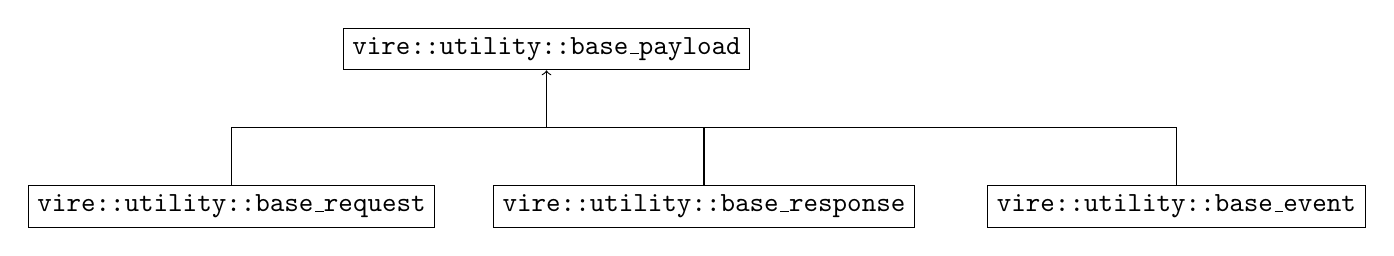
\begin{tikzpicture}
  \node (payload)  at (0,2)  [draw] {\texttt{vire::utility::base\_payload}};
  \node (request)  at (-4,0) [draw] {\texttt{vire::utility::base\_request}};
  \node (response) at (2,0)  [draw] {\texttt{vire::utility::base\_response}};
  \node (event)    at (8,0)  [draw] {\texttt{vire::utility::base\_event}};

  %\draw[style=help lines] (-3,-1) grid (10,4);
  \draw (node cs:name=response,anchor=north) |- (0,1);
  \draw (node cs:name=event,anchor=north)    |- (0,1);
  \draw[->] (node cs:name=request,anchor=north)
  |- (0,1) -| (node cs:name=payload,anchor=south);
\end{tikzpicture}
\end{center}

The requirements for the transmitted object are the following:

\begin{itemize}

\item The  type of the object  must be conventionally associated  to a
  unique     \emph{model      identifier}     object      (see     the
  \texttt{"vire::utility::model\_identifier"} class)  which contains a
  unique   name   (\textit{string    identifier})   and   possibly   a
  \textit{version identifier}.  Each software  component that may send
  or  receive the  object  should agree  on  this type  identification
  scheme.   This   enable  the  use  of   object  factories,  whatever
  programming  langage  is used  on  both  side of  the  communication
  system.

\item  For each  software component,  the object  type must  have some
  dedicated  encoding/decoding  functions  available  (again  whatever
  programming language is used). For example the Vire API supports the
  following encoding formats:

  \begin{itemize}

  \item JSON (MIME  encoding type: \texttt{"application/x-json"}), which
    is supportable by many languages,

  \item  Protobuf  (Google  Protocol   Buffers,  MIME  encoding  type:
    \texttt{"application/x-protobuf"}), which is also widely supported,

  \item   Boost/serialisation   (XML,    text   or   binary   archives
    \texttt{"application/x-boost-serialization-xml"},
    \texttt{"application/x-boost-serialization-text"},
    \texttt{"application/x-boost-serialization-binary"}),    which    in
    principle is supported by C++ only.

  \end{itemize}

  The Protobuf  encoding format will be  used to serialize/deserialize
  the  Vire  messages transported  between  the  Vire server  and  the
  CMS/LAPP server.

\end{itemize}

Vire uses a dedicated layout to represent the body of any message with
its embedded payload object. With this technique, the structure of the
body          contains         two          attributes         (figure
\ref{fig-app-vire-message-message_body-cpp}):

\begin{enumerate}

\item The \texttt{payload\_type\_id} specifies the type of the payload
  object   (figure   \ref{fig-app-vire-utility-model_identifier-cpp}).
  This unique name  is conventionaly fixed for a  given application. A
  version tag allows to support possible evolution of the object type.

\item The  \texttt{payload} is a  handle to  a payload object  of type
  request, response or event.

  %% \begin{itemize}
  %% \item Within  the producer  component of  the message,  the encoding
  %%   function associated to the object  type is responsible to generate
  %%   the JSON stream for the object and store it in the buffer.

  %% \item Within  the consumer  component of  the message,  the decoding
  %%   function associated to the object type is responsible to parse the
  %%   JSON stream stored in the buffer and restore the object in memory.

  %% \end{itemize}

  It is expected  that, on both sides of the  connection, the software
  components can  access dedicated  software plugins which  ensure the
  support  of  various   \emph{payload  object  types}  conventionnaly
  associated  with  their  \emph{payload type  identifiers}  and  also
  providing JSON and/or Protobuf encoding/decoding functionalities.

  %% The   system  allows  to  support
  %% modification  in the  structure of  the objects  thanks to  version
  %% tagging.

\end{enumerate}

\begin{figure}[h]
\vskip 10pt
\small
\begin{Verbatim}[frame=single,xleftmargin=0.cm,label=\fbox{C++}]
struct message_body {
  vire::utility::model_identifier     payload_type_id; // Object type identifier.
  const vire::utility::base_payload * payload;         // Handle to a payload object.
};
\end{Verbatim}
\normalsize
\caption{The structure of a message body object (C++).}
\label{fig-app-vire-message-message_body-cpp}
\end{figure}

\begin{figure}[h]
\vskip 10pt
\small
\begin{Verbatim}[frame=single,xleftmargin=0.cm,label=\fbox{JSON}]
{
  "header" : {
    ...
  },
  "body" : {
    "payload_type_id" : {
      "name" : "vire::message::testing::error_event",
      "version" : {
        "initialized" : false
      }
    },
    "payload" : {
      "timestamp" : "20160930T141743.759085"
      "err" : {
        "code" : 3,
        "message" : "A basic error"
      },
    }
  }
}
\end{Verbatim}
\normalsize
\caption{Example of  a   message  body  object in JSON format.}
\label{fig-vire-message-message_body-json}
\end{figure}

\vfill
\clearpage
\pagebreak

% end
